\section* {3.1}

\subsection{Постановка задачи}
Используя таблицу значений $Y_i$  функции $y=f(x)$, вычисленных в точках   $X_i, i=0,..3$  построить интерполяционные многочлены Лагранжа и Ньютона, проходящие через точки $\{X_i,Y_i \}$ .  Вычислить значение погрешности интерполяции в точке $X^*$. 

{\bfseries Вариант:} 26

$y=1/x^2 + x^2, a)X_i= 0.1,0.5,0.9,1.3;  б)X_i= 0.1,0.5,1.1,1.3; X^* = 0.8$
%\pagebreak

\subsection{Результаты работы}
\begin{figure}[h!]
\centering
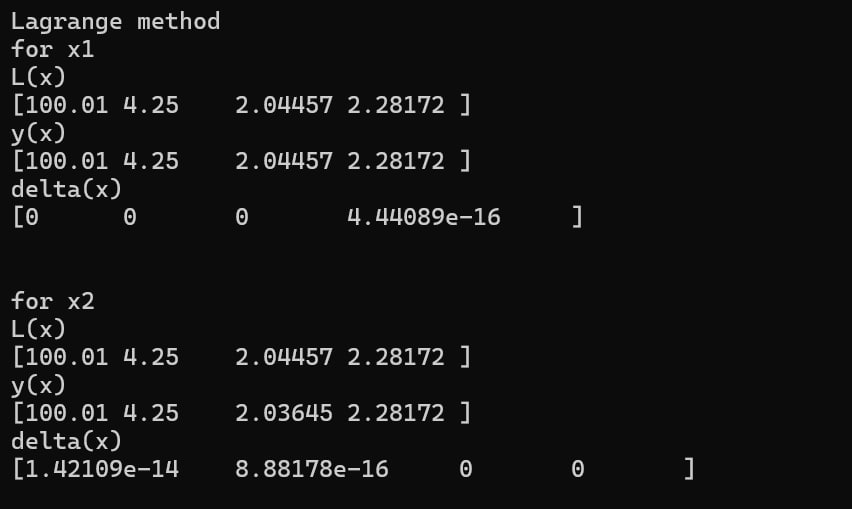
\includegraphics[width=12cm, height=6.5cm]{img1_1}
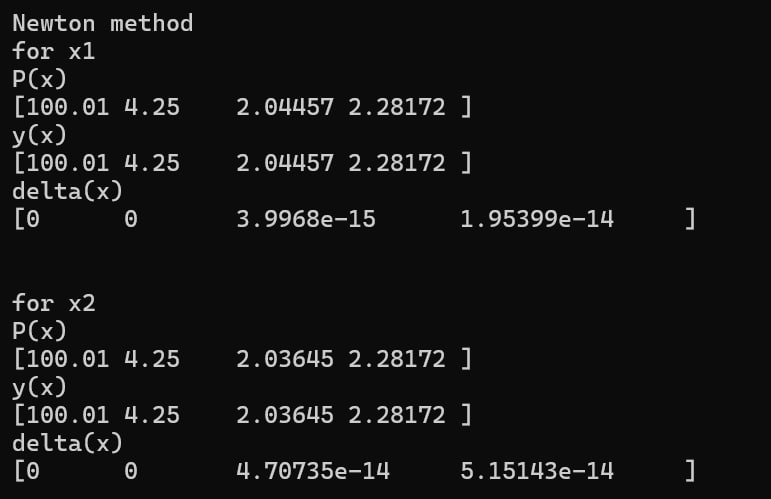
\includegraphics[width=12cm, height=6.5cm]{img1_2}
\caption{Вывод программы в консоли}
\end{figure}
\pagebreak
% \vfill


\subsection{Исходный код}

\lstinputlisting{include/lab3-1.cpp}
\pagebreak

\section* {3.2}

\subsection{Постановка задачи}
Построить кубический сплайн для функции, заданной в узлах интерполяции, предполагая, что сплайн имеет нулевую кривизну при $x=x_0$  и $x=x_4$. Вычислить значение функции в точке $x=X^*$. 

{\bfseries Вариант:} 26
\begin{figure}[h!]
$X_i=0.8$
\centering
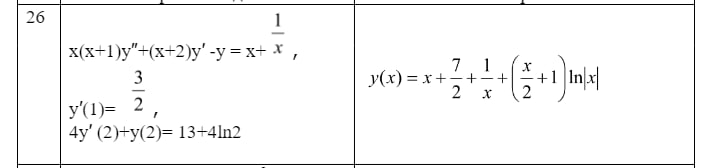
\includegraphics[width=15cm, height=4cm]{img2_1}
\caption{Условие}
\end{figure}
%\pagebreak

\subsection{Результаты работы}
\begin{figure}[h!]
\centering

\includegraphics[width=15cm, height=3cm]{img2_2}
\caption{Вывод программы в консоли}
\end{figure}
\pagebreak

\subsection{Исходный код}

\lstinputlisting{include/lab3-2.cpp}
\pagebreak

\section* {3.3}

\subsection{Постановка задачи}
Для таблично заданной функции путем решения нормальной системы МНК найти приближающие многочлены a) 1-ой  и б) 2-ой степени. Для каждого из приближающих многочленов вычислить сумму квадратов ошибок. Построить графики приближаемой функции и приближающих многочленов.

{\bfseries Вариант:} 26
\begin{figure}[h!]
\centering
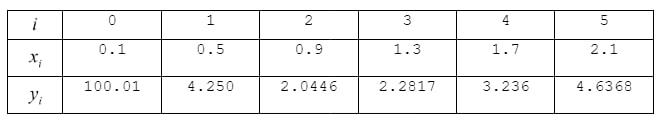
\includegraphics[width=15cm, height=4cm]{img3_1}
\caption{Условия}
\end{figure}
%\pagebreak

\subsection{Результаты работы}
\begin{figure}[h!]
\centering
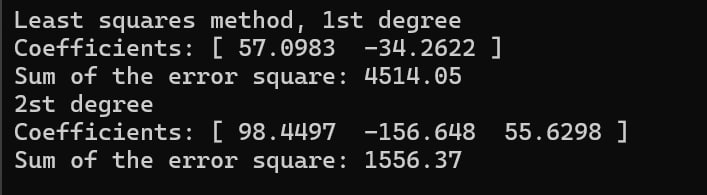
\includegraphics[width=15cm, height=4cm]{img3_2}
\caption{Вывод программы в консоли}
\end{figure}
\pagebreak

\subsection{Исходный код}
\lstinputlisting{include/lab3-3.cpp}
\pagebreak

\section* {3.4}

\subsection{Постановка задачи}
Вычислить первую и вторую производную от таблично заданной функции $y_i=f(x_i), i=0,1,2,3,4$  в точке $x=X_i$.   

{\bfseries Вариант:} 26
$X^*=2.0$

\begin{figure}[h!]
\centering
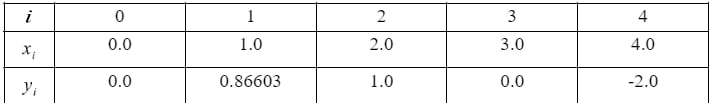
\includegraphics[width=15cm, height=2cm]{img4_1}
\caption{Условия}
\end{figure}
%\pagebreak

\subsection{Результаты работы}
\begin{figure}[h!]
\centering
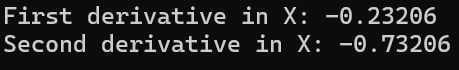
\includegraphics[width=10cm, height=2cm]{img4_2}
\caption{Вывод программы в консоли}
\end{figure}
\pagebreak

\subsection{Исходный код}

\lstinputlisting{include/lab3-4.cpp}
\pagebreak
\section* {3.5}

\subsection{Постановка задачи}
Вычислить определенный интеграл $\int\limits_{X_0}^{X_1} y dx$  , методами прямоугольников, трапеций, Симпсона с шагами $h_1,h_2$. Оценить погрешность вычислений, используя  Метод Рунге-Ромберга: 

{\bfseries Вариант:} 26\\
$y= x^2 \sqrt{36 - x^2}$
$X_0=1, X_k=5, h_1=1.0, h_2=0.5$

\subsection{Результаты работы}
\begin{figure}[h!]
\centering
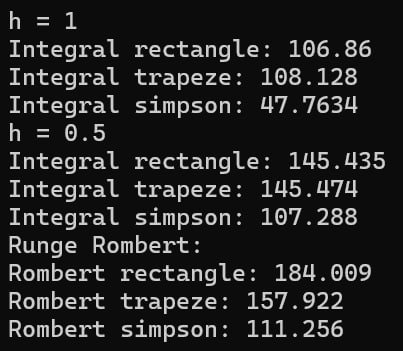
\includegraphics[width=10cm, height=10cm]{img5}
\caption{Вывод программы в консоли}
\end{figure}
\pagebreak


\subsection{Исходный код}
\lstinputlisting{include/lab3-5.cpp}

